\documentclass[]{article}
\usepackage{amssymb,amsmath}
\usepackage{ifxetex,ifluatex}
\ifxetex
  \usepackage{fontspec,xltxtra,xunicode}
  \defaultfontfeatures{Mapping=tex-text,Scale=MatchLowercase}
\else
  \ifluatex
    \usepackage{fontspec}
    \defaultfontfeatures{Mapping=tex-text,Scale=MatchLowercase}
  \else
    \usepackage[utf8]{inputenc}
  \fi
\fi
\usepackage{ctable}
\usepackage{float} % provides the H option for float placement
\usepackage{graphicx}
% We will generate all images so they have a width \maxwidth. This means
% that they will get their normal width if they fit onto the page, but
% are scaled down if they would overflow the margins.
\makeatletter
\def\maxwidth{\ifdim\Gin@nat@width>\linewidth\linewidth
\else\Gin@nat@width\fi}
\makeatother
\let\Oldincludegraphics\includegraphics
\renewcommand{\includegraphics}[1]{\Oldincludegraphics[width=\maxwidth]{#1}}
\ifxetex
  \usepackage[setpagesize=false, % page size defined by xetex
              unicode=false, % unicode breaks when used with xetex
              xetex,
              colorlinks=true,
              linkcolor=blue]{hyperref}
\else
  \usepackage[unicode=true,
              colorlinks=true,
              linkcolor=blue]{hyperref}
\fi
\hypersetup{breaklinks=true, pdfborder={0 0 0}}
\setlength{\parindent}{0pt}
\setlength{\parskip}{6pt plus 2pt minus 1pt}
\setlength{\emergencystretch}{3em}  % prevent overfull lines
\setcounter{secnumdepth}{0}

\title{Example template}
\author{(Username not set) (E-mail address not set)}
\date{2011-04-26 20:25 CET}

\begin{document}
\maketitle

\subsection{Description}

This template demonstrates the basic features of rapport. We all hope
you will like it!

\subsection{Début}

Hello, world!

I have just specified a \emph{Variable} in this template named to
\textbf{leisure}. The label of this variable is ``Internet usage in
leisure time (hours per day)''.

And wow, the mean of \emph{leisure} is \emph{3.1994}!

\subsubsection{Descriptive statistics}

\ctable[pos = H, center, botcap]{lllllll}
{% notes
}
{% rows
\FL
\textbf{Min.} & \textbf{1st
Qu.} & \textbf{Median} & \textbf{Mean} & \textbf{3rd
Qu.} & \textbf{Max.} & \textbf{NA's}
\ML
0.000 & 2.000 & 3.000 & 3.199 & 4.000 & 12.000 & 37.000
\LL
}

The 5 highest values are: \emph{12}, \emph{12}, \emph{10}, \emph{10} and
\emph{10}.

\subsection{Description}

This template demonstrates the basic features of rapport. We all hope
you will like it!

\subsection{Début}

Hello, world!

I have just specified a \emph{Variable} in this template named to
\textbf{leisure}. The label of this variable is ``Internet usage in
leisure time (hours per day)''.

And wow, the mean of \emph{leisure} is \emph{3.1994}!

\textbf{For more detailed statistics, you should have set
\texttt{desc=TRUE}!}

\subsection{Description}

This template demonstrates the basic features of rapport. We all hope
you will like it!

\subsection{Début}

Hello, world!

I have just specified a \emph{Variable} in this template named to
\textbf{leisure}. The label of this variable is ``Internet usage in
leisure time (hours per day)''.

And wow, the mean of \emph{leisure} is \emph{3.1994}!

\textbf{For more detailed statistics, you should have set
\texttt{desc=TRUE}!}

\subsubsection{Histogram}

\begin{figure}[htbp]
\centering
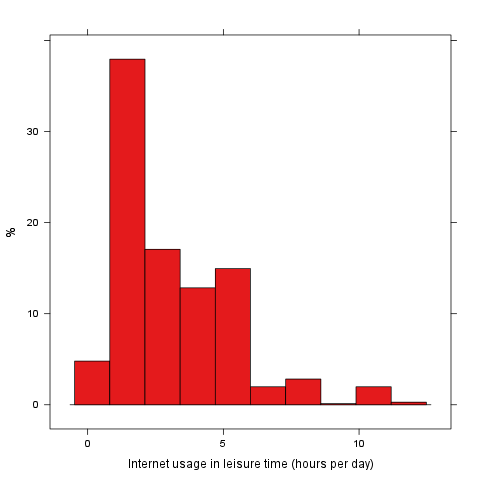
\includegraphics{9542b7929dcd934208ee4f18bde6ff31.png}
\caption{}
\end{figure}

\subsection{Description}

This template demonstrates the basic features of rapport. We all hope
you will like it!

\subsection{Début}

Hello, world!

I have just specified a \emph{Variable} in this template named to
\textbf{leisure}. The label of this variable is ``Internet usage in
leisure time (hours per day)''.

And wow, the mean of \emph{leisure} is \emph{3.1994}!

\textbf{For more detailed statistics, you should have set
\texttt{desc=TRUE}!}

\subsubsection{Histogram}

\begin{figure}[htbp]
\centering
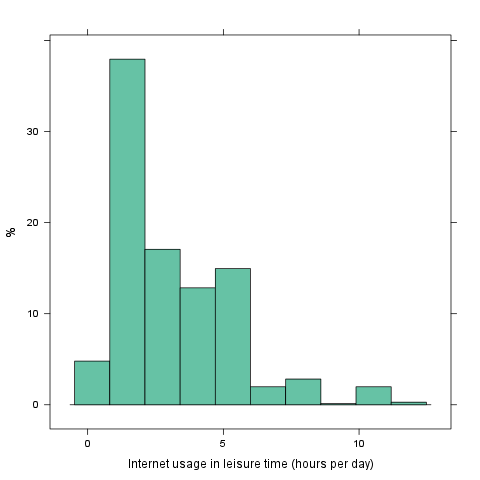
\includegraphics{f72d3b7413bcb88fce740c2ab229411a.png}
\caption{}
\end{figure}

\begin{center}\rule{3in}{0.4pt}\end{center}

This report was generated with
\href{http://rapport-package.info/}{rapport}.

\begin{figure}[htbp]
\centering

\includegraphics{images/rapport.png}
\caption{}
\end{figure}

\end{document}
